\documentclass[11pt]{article}
\usepackage{graphicx}
\usepackage{timeline}
\usepackage{cite}
\usepackage[hang,small,bf]{caption}
\usepackage{fixltx2e}
\usepackage{booktabs}
\bibliographystyle{unsrt}

\begin{document}

\title{Master's thesis proposal [rev\_3]\\
	   \large{Tablet-based dental treatment planning prototype}}
\author{Richard Oldham, DDS\\
		\texttt{rio6@pitt.edu}\\
		Department of Biomedical Informatics\\
		University of Pittsburgh}

\maketitle

\begin{abstract}
The benefits of Computerized Patient Records (CPRs) are well documented. Yet current dental CPRs inadequately support chairside use. Research from the medical informatics literature suggests tablet devices hold promise as an alternative to traditional desktop PCs' ergonomic shortcomings in the clinical environment. If dental professionals have any hope of realizing the advantages of CPR use, information systems must adapt to the user's workflow and not \textit{vice versa}. Designing a mobile treatment planning application for a tablet, which incorporates dental user and usability feedback, may bridge the adoption gap between office and chairside computer use in dentistry. Evaluation can determine if users are faster, more successful, or more subjectively satisfied with the tablet application over traditional CPRs.
\end{abstract}
\tableofcontents
\newpage

\section{Background}
First, I summarize current findings from dental informatics research on CPRs. Next, I discuss current understanding of user models in general dental practice. Lastly, I discuss conclusions and potential solutions from the combined dental and medical literature.

\subsection{Adoption Gap}
\label{Adoption Gap}

The adoption of CPRs by healthcare professionals has long been recognized as a key step in improving patient care\cite{Chasteen1992A-computer-data,Eisne1993The-computer-ba,Thompson2004The-Decade-of-H,Spicer2008Bytes-and-bites,Schleyer2011Advancing-oral}. Dentists have long since recognized the power of computers assisting with practice administration, such as scheduling and billing, and became early adopters of computers in-office (Figure 1).
\label{fig:1}
\begin{figure}[!b]
\begin{center}
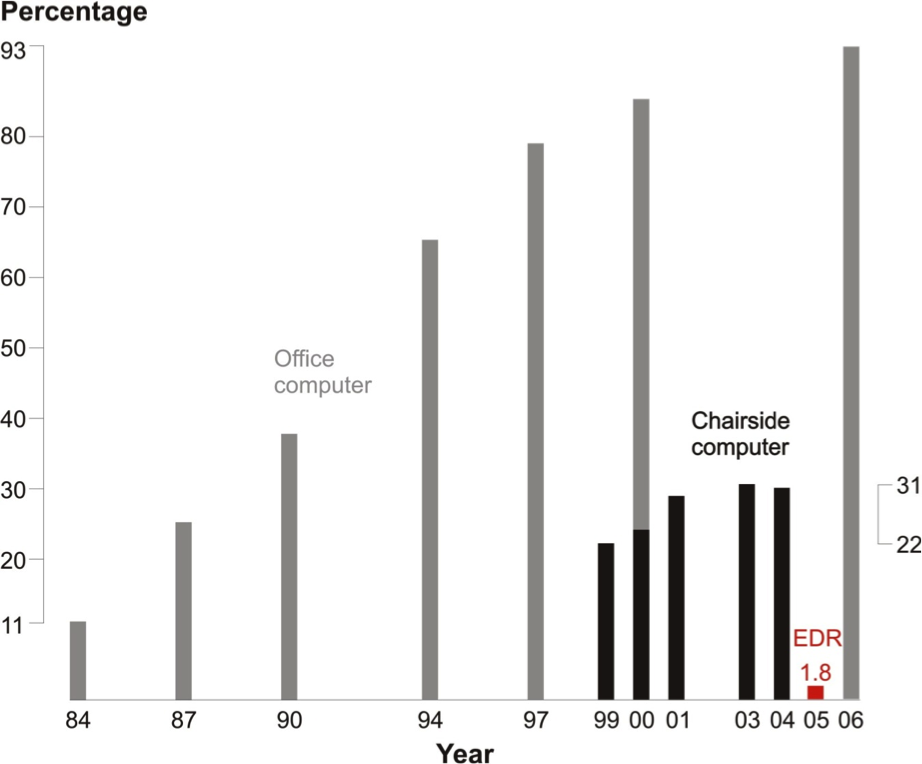
\includegraphics[width=220pt, height=175pt]{comp.png}
\end{center}
\caption{Year of first adoption of computers for office and chairside use in US dental offices\cite{Schleyer2006Clinical-Comput}.}
\end{figure}Survey data from 2010, the most recent available, reports 87\% of respondents using such Practice Management Software (PMS); PMS refers to software that handles office administration whereas CPR software handles a patient's clinical data\cite{Levine2010}. Yet the conclusions of two usability studies on four dental CPRs, which together comprise more than a 70\% market share for such systems, suggest current dental software is poorly designed for supporting chairside use\cite{Thyvalikakath2007Heuristic-evalu,Thyvalikakath2008A-usability-eva}. These conclusions help explain the gap between office adoption of computers and the adoption of computers for chairside use evident in Figure 1.

The first of the two cited usability studies employed heuristic evaluation\cite{Nielsen1994Usability-Inspe} methods. Three evaluators examined each of the four CPRs and tabulated violations of Nielsen's heuristics. 229 heuristic violations were found in total across EagleSoft, Dentrix, PracticeWorks, and SoftDent suggesting the software dentists were using at the time had significant room for improvement. The second usability study compared\cite{Nielsen1994Enhancing-the-e} these same market-leading CPRs by assigning common tasks to novice users and measuring task completion. On average, users were able to correctly complete 43\% of the assigned tasks leading to a similar conclusion: the most commonly used dental CPRs suffered from a steep learning curve and unintuitive interface design.

The results of these two studies helped confirm the hypothesis that the most popular dental CPRs inadequately support chairside workflow. All four systems included in these studies began life as PMS with clinical functions added later. All four employ screen designs that include all input options at once rather than the options needed for the portion of workflow (see Figure 2). Cluttered interfaces cause difficulty in finding functionality\cite{Qian2011Towards-develop}. Dentrix and Eaglesoft, for example, intermixed controls for entering existing conditions and planned procedures on the same palette, confusing users.
\label{fig:2}
\begin{figure}[h!tb]
\begin{center}
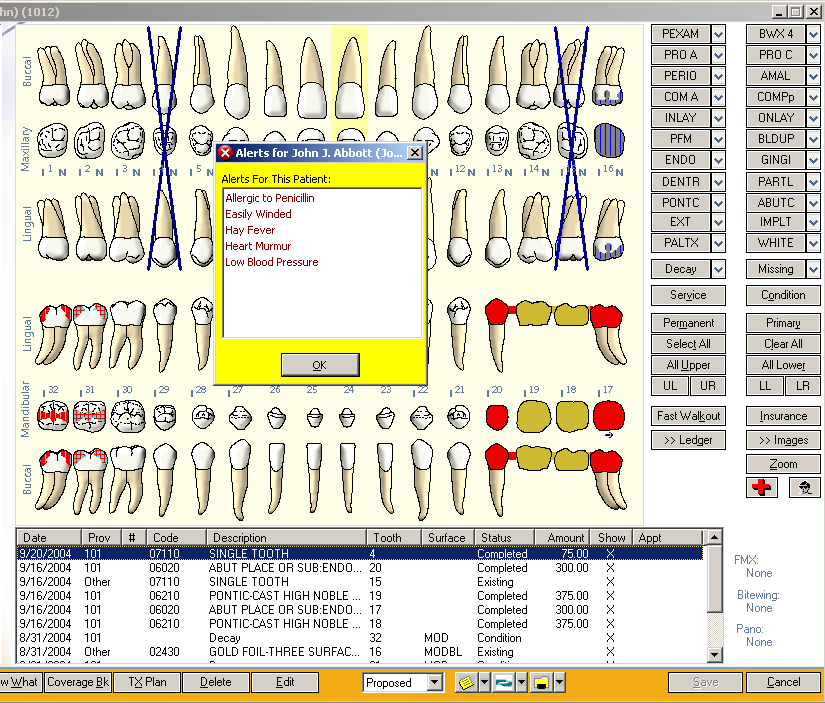
\includegraphics[width=\textwidth]{ss1es.png}
\end{center}
\caption{Screenshot of EagleSoft's user interface.}
\end{figure}Since the information input and retrieval processes are not integrated into the concepts of tasks and workflow, users must divide their attention between navigation and task completion. In both usability studies, the authors noted information that would typically appear on a single paper form was spread out over two or more screens in the CPR. Users experienced difficulty switching between screen views with all systems except PracticeWorks, which has clearly labels tabs adjacent to each other. Evidence suggests these problems are not unique to dental Health Information Technology (HIT) applications\cite{Ash2004Some-unintended,Rose2005Using-qualitati}.

In a telephone survey of 102 general dentists in the United States, researchers discovered three main sources of user frustration in using dental CPRs: poor usability and difficulty entering clinical data\cite{Schleyer2006Clinical-Comput}. Respondents considered ``better input methods,'' ``smaller computers,'' and ``better user interface design'' as principal areas for improvement. Another important concern included lack of infection control inherent with traditional keyboard and mouse input. These responses track closely with those elicited from British users through a similar survey, strengthening the conclusions of both surveys\cite{John2003Questionnaire-s}.

Dental practices use their computers primarily for scheduling patients and tracking completed procedures (Figure 3). This is due, in some part, to the difficulty of integrating the necessary hardware into an already cramped dental operatory\cite{Schleyer2004Why-integration,Unthank2004Designing-your-} and, in some part, to the time-prohibitive cost of entering data into a poorly designed system. The ergonomics of one dentist, one assistant, and one patient gathering, entering, retrieving, and presenting information are complex. The suggested areas of improvement noted in the Schleyer, et al. (2006) survey highlight the frustration of using software designed without these ergonomics in mind. The task of finding the required information inside the patient record is often criticized as time-intensive and distracting\cite{Nygren1998Helping-clinici}. This is especially concerning given the increased complexity of care provided in an increasingly time-pressured environment. If we accept the premise that HIT can improve patient care, and there exists a large adoption gap, the necessity of generating and understanding a user model becomes apparent.

\subsection{User Model}
Recognizing this adoption gap, researchers set out to model the workflow of an initial examination and treatment planning appointment through contextual inquiry\cite{Irwin2009A-preliminary-m}. During this appointment the dentist documents the patients current condition(s), the patients goal for oral health, and generates a sequenced plan to proceed from present state to the goal state. This process, with its findings and resulting plan, must then be discussed with the patient. Depending on the complexity of diagnoses, multiple treatment plans may be required. Of any appointment, this one generates the most clinical artifacts such as radiographs, hard and soft tissue diagnostic charting,  and gypsum study models. Following the initial visit and generation of a treatment plan, each subsequent visit requires comparatively little interaction with the CPR. The dentist may check the medical history or reference the planned procedures, for example. Thus the initial appointment requires the most interaction with the CPR for data entry and retrieval, making it an ideal candidate for study.

A thorough initial exam and treatment planning appointment is vital for not only diagnosing every present condition but communicating the condition, its consequences, and treatment options as well. Watching a seasoned dentist perform the initial exam and treatment plan is analogous to peeling an onion; the dentist starts with the most obvious signs and symptoms and continues examination, testing, and imaging until all signs and symptoms have been mapped to a problem list. The dentist may ascribe diagnoses to items on the problem list and then generate a treatment to address each item. This process is non-deterministic, across patients and dentists, and time-intensive, often requiring two people, one operator to diagnose and one assistant to transcribe the findings into the computerized record. While this task may be handled differently in sequence from one dentist or patient to another, the steps are the same and mappable to common set of terms and abstractions. 

The Dental Information Model (DIM), a blueprint for the content and structure of patient records in general dentistry, is maturing through research collaboration between the Center for Dental Informatics and Marshfield Clinic Biomedical Informatics Research Center\cite{Acharya2009Electronic-dent}. The DIM offers guidance for database design in helping ensure the software system has adequate expressive power\cite{Schleyer2007A-Qualitative-I} in making real world data elements to data fields in the system. Doing so could address the disconnect between the real world and system noted in usability testing and survey data on what types of data are stored on paper and the computer. Further, data interchange is made easier in using a standard DIM. To the extent the interface design must dovetail with the underlying data layer, the DIM is helpful in designing the interface as well.

Faced with the complexity of the initial exam process, most dentists dictate their findings to an auxiliary, who transcribes them into the record. Irwin, et al. (2009) observed an auxiliary may not always be available and dental team members used a variety of workarounds in such a situation. For example, hygienists often perform recare examinations without an assistant, noting their preliminary findings on a piece of paper prior to discussion with the dentist. Even under ideal circumstances, that is, when an assistant was present, over 60\% of the observed breakdowns in this study were due to technology. One implicit conclusion from the Irwin model is dentists spend little time entering data with the majority of CPR interaction handled by hygienists and assistants. Schleyer, et al. (2006) reported dentists participating in only 23\% of data entry tasks, chief among them being progress note entry. Hygienists and assistants handled most other data entry tasks such as diagnoses, oral health status, and histories. Whether dentists would employ more clinical functions in their CPR given improved interfaces, as Irwin, et al (2009) described, ``with the flexibility in sequencing, granularity and comprehensiveness'' for data entry remains to be seen. But the conclusions of Irwin et al. (2009) mirror the conclusions from the Schleyer et al. (2006) survey: if dentists implement use CPRs to improve patient care, the CPR design must accommodate to the demands of dental workflow.

Schleyer et al. (2006, 2007) and Irwin et al. (2009) report the common practice of using multiple or duplicate data entry. A user may write something on paper, such as routing slips or preliminary findings, later transcribing this information into the electronic record. Alternatively, a practice may record the medical history on paper and use the CPR to record planned and completed treatments. This is due, in part, to the fact that dental CPRs lack some date elements and the flexibility present in paper forms\cite{Schleyer2007A-Qualitative-I}. And this is due, in part, to the non-linear and variable process by which patients are escorted through this initial visit. Therefore, an alternative system needs to allow the user a temporary and mutable data store to enter information before committing the entry to the record. And the clinical vocabulary of the information system must be at least as large as that of the clinician. While one can never hope to \emph{a priori} enumerate this vocabulary, allowing the user to customize the type and sequence of information capture may suffice. 

Figure 3 illustrates which types of data are most commonly recorded on paper versus the computer-based record.\label{fig:3}
\begin{figure}[h!t]
\begin{center}
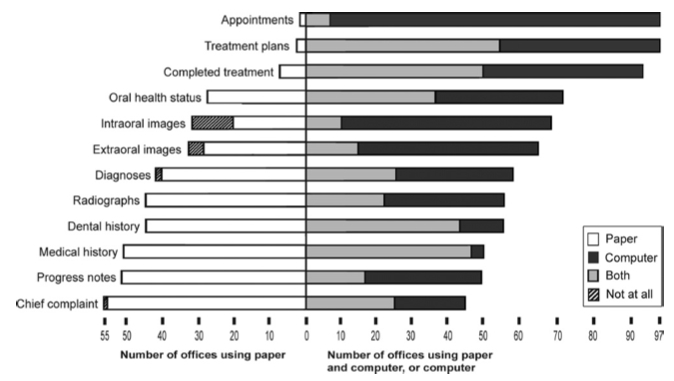
\includegraphics[width=\textwidth]{papervscomp.jpg}
\end{center}
\caption{Storage of major clinical information categories on paper/computer, sorted by utilization of computer-based storage in descending order\cite{Schleyer2007A-Qualitative-I}.}
\end{figure}
While duplicate data entry is not an inherent problem, such a practice has potential for problems. Storing some information in paper format and some in electronic format, similarly, is not \emph{prima facie} poor practice but requires the consumer of the information to switch between the paper-based and computer-based records. Fragmentation of data into multiple or duplicate locations has one inevitable drawback: switching requires the user to remember which piece of information is needed and where this information is located. This burden on the user's memory can slow the data entry process or produce transcription errors\cite{Salvucci2009Toward-a-unifie}.

\subsection{Conclusions and Solutions}
Several important conclusions can be gleaned from the cited literature. First, dental operatories are small and require careful planning to integrate the CPR's supporting hardware. The suggestion of using smaller computers from the Schleyer, et al. (2006) survey reveals user frustration with this integration burden. Next, the current paradigm in dental CPR design and ergonomics requires an auxiliary for efficient data entry. Most dentists are consumers of patient information while hygienists and assistants perform most data entry. Given the results of the user model study, the highest value targets for CPR improvement are the functions used during the initial visit: namely, diagnoses and treatment planning. Lastly, CPRs are poorly adapted to dental workflow and most dental teams accommodate by using multiple or duplicate data entry. For over a decade, dental clinicians have recognized the potential for hand-held computing devices to address the limitations of traditional PCs\cite{Taylor2002Handheld-comput,Jablow2003Your-practice-i}. Given the findings from survey data, usability studies, and contextual inquiry, a paradigm shift is necessary.


\subsection{Tablets and Usability}
Not everyone agrees on the virtues of tablet adoption\cite{Kaneshige2011iPad-in-Healthc,Mashman:2011uq} and, compared to the medical literature, few investigators have studied tablet use by the dental team\cite{Frank2010IPad--tool-or-t}. Applying the insights from medical informatics research to dental problems presumes exchangeability of the findings. This may not be the case. Physician and dentist workflows have differences (Table 1). A key difference to note is the small number of diagnoses in dentistry compared to medicine; dentists cover a smaller portion of the body compared to physicians. Conversely, for each diagnoses, there are a larger number of choices for treatment in dentistry compared to medicine. One might explain this difference by pointing to the larger role patient preferences play in dental treatment planning\cite{Kay1992Restorative-tre} or the smaller role of evidence-based practice in dentistry compared to medicine\cite{Tellez-2011-Sealants}. Another key difference is ergonomic: physicians stand or sit bedside while the dental ergonomic is unique. Fewer similarities exist, however. The basic tasks of examining, diagnosing, recording findings, notes, and orders are common to both domains.
\begin{table}[h!b]
	\begin{center}
����\begin{tabular}{l l l}
\hline
							&	Dentistry 				& 	Medicine 		\\ \hline
Patient		 				&	Usually not sick			&	Usually sick 	\\
Life \& death				&	Seldom					&	More often		\\
No. of patient encounters	&	Few						&	Many				\\
No. of diagnoses				&	Few						&	Many				\\
No. of therapies/diagnoses	&	Many						&	Few				\\
Initial visit 				&	Many artifacts			&	Fewer artifacts	\\
Average visit length			&	Long						&	Short			\\
Care setting size			&	Small					&	Large			\\
Treatment type				&	Mechanical/ biological	&	Biological		\\
\hline
\end{tabular}\caption{Summary of differences across dental and medical workflows.}\end{center}\end{table}

Tablets offer several advantages over traditional desktop PCs in clinical use. Tablets' smaller size and portability, for instance, were key to driving adoption in medicine as most exam and hospital rooms do not have a CPR access. Likewise, tablets' smaller footprint could help tackle the ergonomic challenges in dental practice. Tablets can at least match the traditional desktop PC in data entry speed and accuracy with use\cite{Kirby1996The-PEN--PAD-da,Mackenzi2002Text-entry-for-}. They can be easily shared between providers or the provider and patient and they can be easily disinfected\cite{Mayrhofer2007Pen-based-Elect}. Properly designed touch-screen mobile interfaces have demonstrated promise in a variety of medical settings\cite{Haller2009Handheld-vs.-la,Mulligen1998Clinical-data-e,Baumgart2005Personal-digita,Lu2005A-review-and-a-,Seneviratne2010Improving-stylu}. Finally, if users are as capable on a mobile device as a traditional PC, the ergonomic and portability advantages can increase user subjective satisfaction with a mobile system over a conventional desktop\cite{Cole2006A-comparative-s}.

Creating a usable and useful interface for the tablet is a separate consideration. Regarding screen design, Thyvalikakath, et al. (2008) recognized the disconnect between task flow and screen design in dental CPRs ahead of a formal modeling study. Several topical conclusions the 2008 comparative usability study include: \begin{itemize}
\item Users should be able to identify their approach to treatment and the system should help support that approach.
\item Data entry and retrieval controls available on screen should correspond with the tasks to be completed, and unrelated or extraneous controls should not be shown. Information that belongs to a specific task context should be shown together or be easily accessible; for instance, hard-tissue and periodontal findings often must be reviewed together to make a clinical decision and should not be separated unnecessarily.
\item Data entry and functional controls should be organized and labeled clearly, given the multitude of input classes (findings, planned/completed procedures, notes, pictures, annotations, to name a few).
\end{itemize}

Lastly, the User-Centered Design (UCD) approach to software engineering has demonstrated promise in general\cite{Bannon1986Issues-in-desig,Wixon1997The-usability-e,Gould1997How-to-design-u,Abras2004Encycolopeida-o} and HIT specifically\cite{Johnson2005A-user-centered}. UCD is a broad term to describe design processes in which end-users influence the software design. Linking the iterative design process to feedback from users has a proven track record. I elaborate on the proposed incorporation of the UCD approach in section 2.2.

\section{Proposed Research}
Based on the results of contextual inquiry and survey research, tablet devices make a logical hardware choice. Hypotheses about clinical tablet use in dentistry remain untested. The extent to which tablet devices and touch interfaces can improve data entry and user satisfaction is a question left to evaluation. But first a working tablet-based treatment planning prototype is required.

Research is currently underway to determine how dentists use their current CPRs. Given the time constraints of dental practice and poor usability demonstrated by market-leading CPRs in evaluation, our hypothesis is most dentists document only planned procedures and few diagnostic findings. This is accepted practice by third-party payers, in contrast to medicine, but is not ideal.

\subsection{Treatment Planning Prototype}

Justify 3 things for functional spec. High value?
Consistent with Jeannie's findings?
Small number of rules to unambiguously and programatically render dx from pl

Many options are available for mobile development. The two dominant operating systems for tablet devices are Android and iOS. To develop a platform-native application, Android requires application coding in Java and iOS requires coding in Objective-C. Alternatively, a web-native application can be ``wrapped'' for use on any platform using responsive web design (a small JavaScript instruction set to resize content based on browser resolution). While each platform has advantages and disadvantages, no design decision has yet been made.

The functional specification includes:

\begin{itemize}
\item The ability to document the most common diagnostic findings in a clinically linear fashion (find all sites affected with diagnostic condition, move on to the next condition)
\item The ability to automatically generate diagnoses from the documented findings
\item The ability to automatically map a list of treatments, based on provider preferences, from the list of problems and diagnoses
\item The ability to bin and sequence the list of treatments to form one or several treatment plans
\end{itemize}

Following the generation of a treatment plan (or plans), the provider next discusses the findings with the patient. The ability to summarize findings for the providers use in treatment planning is as important as communicating these findings to the patient. Using the treatment plan ``patient view'' to facilitate this discussion could help drive treatment plan acceptance. This feature would undoubtedly be beneficial but may fall outside the scope of this project. The ``patient view'' function is but one example of the many functions available to users once patient data is present in the CPR. However, addressing the problem of cumbersome data entry is a necessary prerequisite to reaping the benefits of computerized records.

\subsection{Evaluation}

Evaluation of the tablet application requires comparing it to an alternative. Two logical points of comparison are the most popular CPRs in private practice: Dentrix and EagleSoft. Access to these CPRs has been granted to the CDI and using them for the purposes of evaluation should present no challenges.

Similar to Thyvalikakath, et al. (2008), summative measures like task completion provides a valuable evaluation metric. Task completion time and subjective user satisfaction\cite{Chin1998Development-of-} are also useful. Task completion time can be simply measured with a stop watch by an observer. Subjective user satisfaction could be measured through a survey administered after each user completes the task set on each system. By using within-subjects comparison, the effect of user familiarity with tablet devices and the traditional CPR can be minimized. A pre-observation survey of user comfort and familiarity with the two systems may help explain differences across users.

One important tradeoff to consider is fidelity to real-world use versus ease of evaluation. Setting up a mock clinic with myself (or someone else) acting as a patient would provide a more realistic environment but may bias the evaluation if the primary investigator serves also as the mock patient. Alternatively, several na\"{i}ve users could complete a common task set using the tablet application and an alternative.

As previously described, the UCD approach to development is ideally suited to the proposed research. The University of Pittsburgh's Center for Dental Infromatics and School of Dental Medicine can provide ready access to potential participants for design feedback ahead of the formal evaluation. The purpose of this feedback is to confirm the design specification and to maximize application usability. Depending on the results of this feedback, one or more rounds of iteration may be necessary.  

\section{Proposed Timeline}



\begin{timeline}{2in}(5,70)
\optrule
  \item[10]{April}{Complete proposal}
  \item[14]{April}{Begin thesis}
  \item[18]{May}{Begin development}
  \item[32]{September}{Complete initial prototype}
  \item[35]{September}{Preliminary feedback}
  \item[39]{September}{Iterate on design}
  \item[43]{October}{Begin evaluation}
  \item[57]{November}{Complete evaluation}
  \item[67]{December}{Complete thesis}
\end{timeline}%% Needed comment
\\

\footnotesize{
\bibliography{Master}}

\end{document}